\section{Introduzione}

L'elettronica è la scienza e la tecnica inerente 
alla propagazione ed emissione degli elettroni nel vuoto o nella materia.

\subsection{Legge di Moore}
Il numero di transistori integrati nei chip raddopia ogni due anni.

\subsection{Trasduttore}
\begin{itemize}
    \item sensore: produce un segnale elettrico per una certa grandezza fisica
    \item attuatore: produce una certa grandezza fisica per un segnale elettrico
\end{itemize}

\subsection{Segnale}
Funzione del tempo che rappresenta la variazione di una grandezza fisica.

\subsubsection{I segnali elettrici}
Possono essere analogici(livelli continui nel tempo) o digitali(livelli discreti).

\subsection{Circuiti digitali}
\begin{figure}[H]
    \centering
    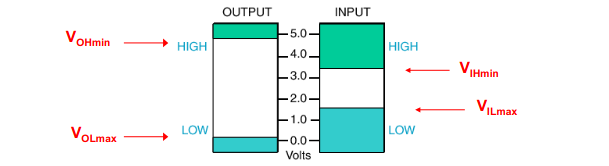
\includegraphics[width=0.5\linewidth]{imgs/0 - livelli-input-output}
    \caption{Livelli input output}
    \label{fig:input_output_livelli}
\end{figure}

\begin{itemize}
    \item $V_{OHmin}$ è la minima tensione in output corrispondente ad un 1 logico
    \item $V_{OLmax}$ è la massima tensione in output corrispondente ad un 0 logico
    \item $V_{IHmin}$ è la minima tensione per avere un 1 logico
    \item $V_{ILmax}$ è la massima tensione per avere un 0 logico
    \item I margini di rumore sono $V_{OHmin} - V_{IHmin}$
    \item I margini di rumore sono $V_{ILmax} - V_{OLmax}$
\end{itemize}

\subsection{Digitale vs Analogico}
\begin{itemize}
    \item elevata potenzialità di calcolo ed elaborazioni del segnale
    \item maggior robustezza a disturbi e rumore
    \item minor sensibilità alle variazioni di temperatura ed alle tolleranze dei parametri del dispositivo
\end{itemize}

\subsection{Analogico vs Digitale}
\begin{itemize}
    \item in natura le grandezze sono continue(segnali analogici)
    \item sensori: grandezza fisica -> ingresso analogico
    \item attuatori: segnale -> uscita analogica
    \item si usano circcuiti di conversione A/D e D/A
\end{itemize}
\subsubsection{ADC}
Converte un input analogico ad un output digitale, si fa una approssimazione dell'input con il
campionamento.

\subsubsection{DAC}
Converte digitale verso analogico.
